\subsection{Architecture (WIP)}
One of the important aspects of this study is to construct such an architecture that allows for the comparison of results between different models. Since the quality of predictions of models composed of various embedding methods and classification algorithms is being compared, it is necessary to ensure that the entire process is designed correctly. The individual variants of embeddings should be trained on the same data, and the classification algorithms on the same embeddings. Figure~\ref{methodology-schema_extended} illustrates the architecture designed for the purpose of comparing the results of the models in this study.

\begin{figure*}
\centering
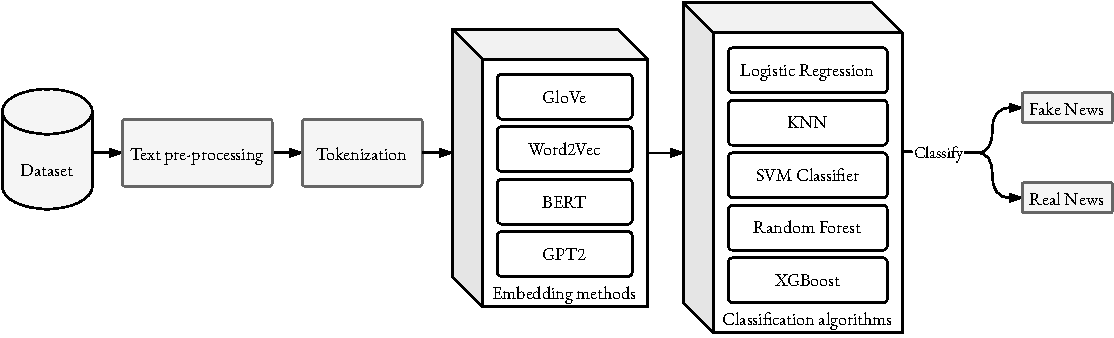
\includegraphics[width=0.8\linewidth]{methodology-schema_gpt2_extended.pdf}
\caption{Architecture of each embedding-classifier model combination}
\label{methodology-schema_extended}
\end{figure*}

The prepared dataset, previously subjected to cleansing and tokenization, has been divided into a training and testing set (further details regarding the dataset's characteristics are provided in the subsequent section). Subsequently, the data underwent an embedding procedure. The same combination of data was employed for all embedding methods utilized.

The Word Embeddings obtained in the previous step served as input for the classification algorithms in the subsequent step. After each word embedding procedure, each algorithm received exactly the same set of data. Hyperparameter tuning on the training set was performed using cross-validation with random search.

Finally, all combinations of 5 embedding methods and 6 classification methods resulted in 30 different fake news detection models. For each embedding-classifier combination, text classification into fake news and real news was performed on the test set created in the first step. More details about the obtained results will be presented in the Results section.


\subsection{Dataset (WIP)}
Access to high-quality data is a significant challenge faced in data modeling and machine learning. In the absence of high-quality data, it is impossible to construct accurate machine learning models. Poor quality data, characterized by unreliable data collection methods, a large number of errors, incompleteness, or mislabeling, can compromise the effectiveness of any machine learning algorithm. This issue is particularly pertinent in the context of datasets containing fake news, where labeling is not as straightforward as with other datasets. The task of manual labeling, which is required to obtain ready-made texts labeled as fake news or real information, can be both time-consuming and challenging, requiring substantial trust in the person performing the labeling. As such, the labeling process is prone to significant human error, which can impact the selection of an appropriate dataset.

This research article aims to investigate how the use of various natural language processing (NLP) methods influences the accuracy of fake news prediction, rather than building a model to accurately predict fake news. Therefore, when selecting a dataset, the most crucial considerations are the quality of the labeled observations and the consistency of the labeled texts across the entire dataset. Additionally, the text should closely align with the research area, as the focus of this study is on detecting fake news. To construct a universal tool for detecting fake news, the dataset should include varied topics and text characteristics, reflecting the real-world distribution as accurately as possible. In this way, the model can learn from natural data, picking up the nuances present in different texts, such as writing style, formality, and topics. However, as noted earlier, the primary objective of this article is not to construct a ready-made tool but rather to examine and impact the predictive quality of different NLP methods. 

\textit{The dataset chosen to carry out the research, which meets the criteria outlined above for a good dataset, is \href{https://www.kaggle.com/datasets/clmentbisaillon/fake-and-real-news-dataset}{\textit{Fake and real news dataset}}, obtained from the Kaggle website. The dataset comprises 40,000 observations, encompassing both authentic and fake news articles. Each observation is characterized by five variables that explicate the news item, namely, the news item's title, its content, the topic it pertains to, the date of publication, and a binary label denoting if the news is fake or not. Notably, the dataset is balanced, containing an equivalent number of true and fake news items.}

\hl{Do zrobienia: zrobic reasearch o datasecie, z duzym prawdopodobienstwem ten dataset jest slaby, poszukac lepszego, nastepnie lepiej opisac dane niz w tym przypadku, skad sa i takie tam}

The raw dataset underwent a process of data cleaning and feature engineering. The topics of the news articles were concatenated with their respective content, resulting in a longer text that retains all pertinent information. The cleaned texts were further processed by removing stopwords and punctuation marks. The topic information was omitted from the analysis as it unnecessarily complicates the dataset, potentially introduces uncertainty regarding its correctness, and is difficult to obtain for new data. Importantly, introducing additional variables would add noise to the prediction results, thereby complicating the analysis of the impact of different embedding methods on prediction accuracy. Similarly, the time variable of article publication was also omitted. The resulting dataset is now ready for further analysis and for applying embedding techniques to the news content.


\subsection{Embeddings (WIP)}
The next step after cleaning the data is to convert it in a way that is understandable to the computer. Textual data have the characteristic of forming a coherent whole. Individual letters form words, words form sentences, and sentences form longer pieces of text with a logical structure. Natural language is full of nuances. The same words can have different meanings and emotional connotations depending on the context. Understanding language comes naturally to humans and does not pose major difficulties. The human brain easily captures the appropriate context of words and their meaning, combining them into a logical and coherent text.

However, computers operate in a completely different way than the human brain. Computers are only capable of analyzing sequences of bits, which when arranged in a specific order, yield a result in the form of an element of a larger whole. This way, a sequence of bits can be presented as individual letters. Further, a sequence of letters can be represented as words. Then, in the tokenization process, individual words can be assigned a specific number. This way, the computer is able to decode the data represented by these words into something it can understand.

Nevertheless, the problem of conveying a deeper understanding of the text, the meaning of individual words, and the semantic relationships between them as understood in terms of similarity and analogies, still remains to be solved. The answer to this problem is Word Embedding. Word Embedding is used to represent words using numerical vectors, in such a way that the distance calculated between two words that are semantically similar is small, and between two semantically different words is large.

The Figure~\ref{embedding_example} illustrates the graphical interpretation of Word Embedding, often encountered in the literature. Similar words, such as King and Queen, Man and Woman, are closer to each other in the vector space. Two dimensions can be interpreted. The first dimension determines the fact of being a member of the family, while the second dimension indicates gender.

\begin{figure}[hbt!]
\centering
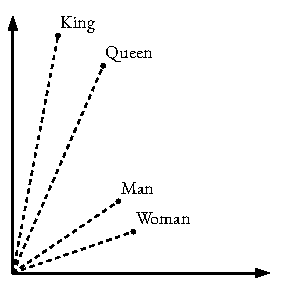
\includegraphics[width=0.55\linewidth]{embedding_example.pdf}
\caption{Similar words are closer together}
\label{embedding_example}
\end{figure}

Trained unsupervised machine learning algorithms handle the conversion of words into vectors from large sets of textual data. These algorithms learn to predict the context of a given word by analyzing the words with which it is associated. In this process, they learn the context of words and the semantic relationships between them. Examples of such algorithms include BERT, Glove, Word2Vec, and GPT-2, which has not yet been investigated in the literature for the purpose of fake news detection.

\subsubsection{GloVe}
GloVe (Global Vectors) is an unsupervised machine learning algorithm aimed at creating word embeddings by aggregating co-occurrence matrices of words that contain information about how often individual word pairs occur in a given text corpus.

The starting point is to create a co-occurrence matrix. The values in this matrix indicate how often a given word pair occurs together. The next step is to calculate the probability of one word occurring in the presence of another word, or rather the ratio between successive probabilities \autocite{Pennington2014}. Without delving into mathematical details, word embeddings are obtained using a matrix subjected to factorization in a process similar to dimensionality reduction \autocite{Albrecht2020}.

It is possible to use pre-trained word vectors trained on large text datasets. In this paper, a model trained on Common Crawl was used, consisting of 840 billion tokens and 2.2 million words, which allowed for obtaining 300-dimensional vectors for each word.

\subsubsection{Word2Vec}
The Word2Vec algorithm is yet another method for obtaining word embeddings. Unlike GloVe method, it is not a method that consists of a single, homogeneous algorithm. Word2Vec can be based on two distinct models: the CBOW and Skip-Gram Model.

The functioning of these two algorithms can be intuitively interpreted as two opposites. CBOW works as a model that predicts a given word based on its context. On the other hand, the Skip-Gram Model is a model that predicts the context of a given word, i.e., the words preceding and following it. Both models are built on a 3-layer neural network with an input layer, a hidden layer, and an output layer.

The originator of the Word2Vec method recommends using the Skip-Gram Model with negative sampling, which outperforms other variants in research. In this study, pre-trained vectors were used, trained on a portion of the Google News dataset consisting of about 100 billion words. The model consists of 300-dimensional vectors for 3 million words and phrases. It was not specified which Word2Vec method was used to obtain these vectors \autocite{Mikolov2013}.

\subsubsection{BERT}
BERT (Bidirectional Encoder Representations from Transformers) is a deep learning Large Language Model founded on the transformer self-attention mechanism. The transformer architecture incorporates encoders responsible for assimilating input data and assigning importance weights to individual words via the self-attention mechanism. This allows BERT to acquire an understanding of contextual dependencies among words within a sentence. Unlike sequential directional models, which process textual input data in a linear fashion, transformer encoders simultaneously process all words, resulting in an inherently bidirectional nature \autocite{Vaswani2017}. The bidirectional sentence-level classification architecture of BERT is depicted in the provided Figure~\ref{bert_architecture}.

\begin{figure}[hbt!]
\centering
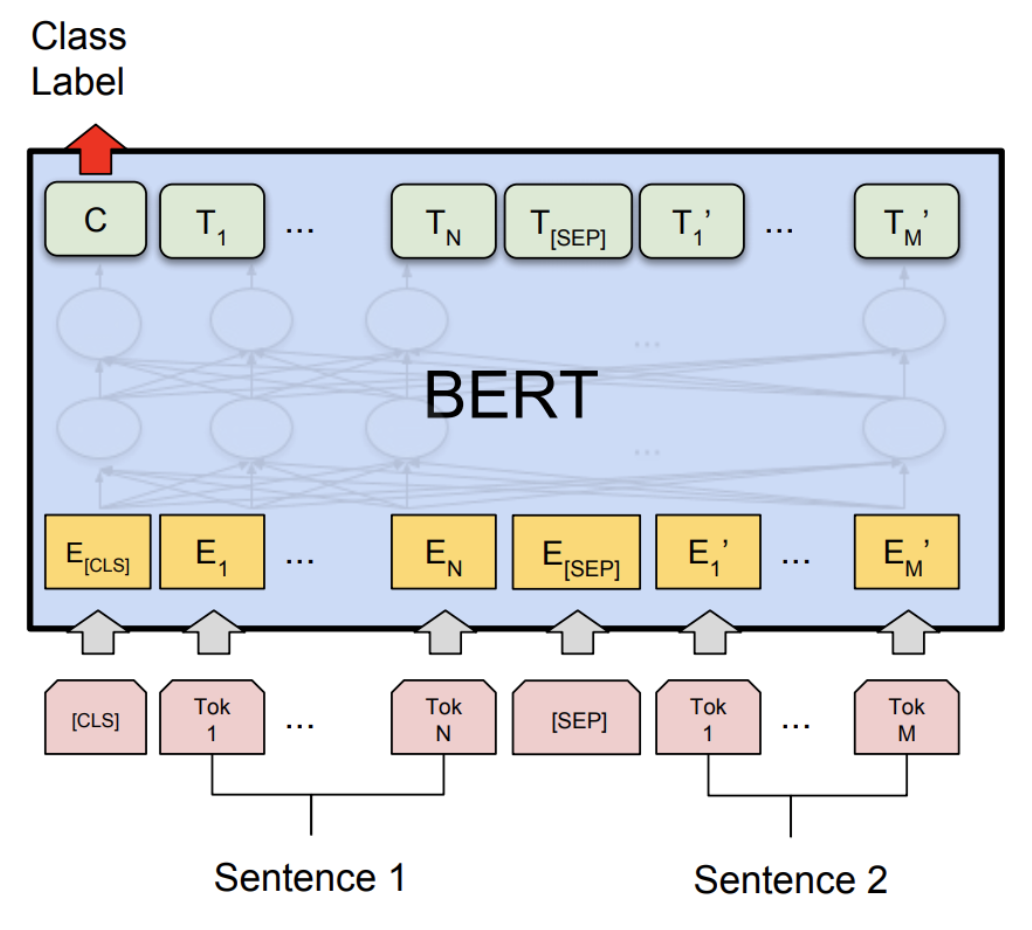
\includegraphics[width=0.75\linewidth]{bert_architecture.png}
\caption{BERT model architecture \autocite{Devlin2018}}
\label{bert_architecture}
\end{figure}

BERT belongs to the class of masked language models. This implies that the learning process of BERT can be interpreted in such a way that the model randomly masks a selected word and, based on the surrounding words (both preceding and succeeding), predicts the masked word using the mechanisms described earlier. 
Next Sentence Prediction (NSP) serves as another objective for the model during the pre-training process. In this procedure, BERT combines two randomly masked sentences as inputs. Subsequently, the model generates predictions regarding whether the given pair of sentences logically follows each other or not.

A noteworthy characteristic of BERT is its pre-training capability. During the pre-training phase, the BERT model acquires contextual understanding of a given word by analyzing the surrounding words. This is achieved through the application of a masked language model (MLM), where tokens are randomly masked, and the model attempts to predict the missing word's semantics. BERT offers a variety of pre-trained models that can be utilized for diverse purposes. Specifically, the BERT-base model, employed in this study, encompasses 12 encoder stack layers, 768 hidden units, and 12 multi-head attention heads, comprising a total of 110 million parameters. The pre-training of this model was conducted on a dataset containing 11,038 books and the English edition of Wikipedia.

BERT requires input data to be specially converted to the required format before being used in the pre-trained model. This enables the use of its key component, word embedding. During word embedding, BERT uses a technique called WordPiece. This technique is based on breaking words down into smaller subwords. This is done to capture the meanings of words that may have different interpretations or different meanings depending on the context. The WordPiece technique thus creates all combinations that can occur in a given text, assigning each extracted part a pre-trained vocabulary vector. These vectors then serve as input data for the previously trained transformer architecture.

An important feature of BERT is the fact that it can be fine-tuned for use in a specific task or adapted to the characteristics of a given dataset. Fine-tuning involves running the pre-trained model training on a new dataset for several epochs. According to the literature, such a trained model achieves state-of-the-art performance. However, in this paper, I will not be performing fine-tuning. Instead, I focus on comparing the impact of using different embedding methods on changes in model performance. Additionally, as mentioned earlier in the literature review, fine-tuning can be replaced by using a classifier on the pre-trained BERT architecture.

In this research, I use BERT as a feature extractor. I extract embeddings for the first token ([CLS] token) from the last hidden layer of the model.

\subsubsection{RoBERTa}
The Robustly Optimized BERT Approach (RoBERTa) is a modification of the BERT model. The creators of the model have modified the way in which the input data is masked. In the case of BERT, masked words were inputted to the model as input data. This is a weakness because during the training of the model in successive epochs, the model learned from the same duplicated data. RoBERTa introduces a change in the form of dynamic token masking during training in successive epochs. Additionally, another change introduced in RoBERTa is the removal of Next Sentence Prediction (NSP) during pre-training. The remainder of the architecture is identical to that of the BERT model.
Furthermore, RoBERTa is trained on a larger amount of data (160GB corpus text, with 16GB of the same data used for training BERT).
Due to the improvements made, RoBERTa is expected to demonstrate better performance than BERT \autocite{Liu2019}.

\subsubsection{GPT-2}
Another model utilizing the transformer architecture is the GPT-2 (Generative Pre-trained Transformer 2) model. Unlike BERT, it does not process input data in two directions but rather employs a unidirectional architecture that reads data from left to right. Another distinction is that GPT-2 utilizes decoder-only transformers (while BERT employed encoder-only transformers). This difference arises from the distinct purposes of the models. BERT was designed as a tool to create various models for different applications at a low cost by adding an additional layer. Consequently, BERT employs encoders whose output comprises contextualized embeddings that can serve as inputs for further models. On the other hand, GPT-2 serves an entirely different purpose, which is text generation. Since the model's output should be comprehensible to humans, GPT-2 relies solely on decoder-only transformers.

Decoders in GPT-2, similar to BERT, employ self-attention mechanisms. However, unlike BERT, self-attention in GPT-2 only takes into account preceding words. Otherwise, if considering the subsequent words in the sequence, the model would incorrectly learn to predict the next word by simply returning the next word in the sequence with the highest probability of occurrence. Another difference between GPT-2 and BERT lies in the fact that GPT-2 processes data token by token (while BERT processes the entire text simultaneously). GPT-2 generates predictions for the next word based on the preceding text. The output of one iteration simultaneously serves as the input for the next iteration.


\subsection{Classification algorithms (WIP)}
\textit{Describe what classification algorithms has been used and what are the pros and cons for each of them...}

\subsubsection{Logistic Regression}
\textit{Description of Logistic Regression algorithm...}

\subsubsection{K-nearest neighbors algorithm (KNN)}
\textit{Description of KNN algorithm...}

\subsubsection{SVM Classifier}
\textit{Description of SVM Classifier algorithm...}

\subsubsection{Random Forest}
\textit{Description of Random Forest algorithm...}

\subsubsection{XGBoost}
\textit{Description of XGB algorithm...}

\subsubsection{Neural Network}
\textit{Description of Neural Network algorithm...}
\\
\hl{Do zrobienia: polepszyc tunowanie NN, upewnic sie ze nie ma bledow w kodzie}

\subsection{Metrics (WIP)}
\textit{Description of used performance metrics..}



\subsection{Results (WIP)}

\begin{table}[hbt!]
\begin{threeparttable}
\caption{GloVe Embeddings results}
\label{glove_embeddings_results}
\begin{tabular}{lll}
\toprule
\headrow Model & Accuracy & F1-Score\\
\midrule
 \textbf{Logistic Regression}                &       \textbf{98.5} &       \textbf{98.4} \\
 KNN               &       92.5 &       92.0   \\
 \textbf{SVM Classifier}               &       \textbf{98.5} &       \textbf{98.4} \\
 Random Forest      &       93.5 &       93.2 \\
 XGBoost           &       96,0   &       95.7 \\
 Neural Network     &       92.5 &       91.4 \\
\bottomrule
\end{tabular}
%\begin{tablenotes}[hang]
%\item[]Table note
%\item[a]First note
%\item[b]Another table note
%\end{tablenotes}
\end{threeparttable}
\end{table}

\begin{table}[hbt!]
\begin{threeparttable}
\caption{Word2Vec Embeddings results}
\label{word2vec_embeddings_results}
\begin{tabular}{lll}
\toprule
\headrow Model & Accuracy & F1-Score\\
\midrule
 Logistic Regression             &       98.0   &       97.9 \\
 \textbf{SVM Classifier}            &       \textbf{98.5} &       \textbf{98.4} \\
 KNN            &       89.0   &       87.8 \\
 Random Forest &       94.5 &       94.1 \\
 XGBoost        &       96.0   &       95.6 \\
 Neural Network  &       97.5 &       97.3 \\
\bottomrule
\end{tabular}
%\begin{tablenotes}[hang]
%\item[]Table note
%\item[a]First note
%\item[b]Another table note
%\end{tablenotes}
\end{threeparttable}
\end{table}

\begin{table}[hbt!]
\begin{threeparttable}
\caption{BERT Embeddings results}
\label{bert_embeddings_results}
\begin{tabular}{lll}
\toprule
\headrow Model & Accuracy & F1-Score\\
\midrule
 Logistic Regression                 &       96.5 &       96.2 \\
 KNN                &       95.5 &       95.2 \\
 \textbf{SVM Classifier}                &       \textbf{97.5} &       \textbf{97.4} \\
 Random Forest       &       94.0   &       93.8 \\
 XGBoost            &       95.5 &       95.3 \\
 Neural Network      &       95.5 &       95.3 \\
\bottomrule
\end{tabular}
%\begin{tablenotes}[hang]
%\item[]Table note
%\item[a]First note
%\item[b]Another table note
%\end{tablenotes}
\end{threeparttable}
\end{table}

\begin{table}[hbt!]
\begin{threeparttable}
\caption{RoBERTa Embeddings results}
\label{roberta_embeddings_results}
\begin{tabular}{lll}
\toprule
\headrow Model & Accuracy & F1-Score\\
\midrule
 \textbf{Logisitc Regression}              &      \textbf{100}   &      \textbf{100}   \\
 KNN             &       99.0   &       98.9 \\
 \textbf{SVM Classifier}             &      \textbf{100}   &      \textbf{100}   \\
 Random Forest    &       98.0   &       97.8 \\
 \textbf{XGBoost}         &      \textbf{100}   &      \textbf{100}   \\
 \textbf{Neural Network}   &      \textbf{100}   &      \textbf{100}   \\
\bottomrule
\end{tabular}
%\begin{tablenotes}[hang]
%\item[]Table note
%\item[a]First note
%\item[b]Another table note
%\end{tablenotes}
\end{threeparttable}
\end{table}

\begin{table}[hbt!]
\begin{threeparttable}
\caption{GPT-2 Embeddings results}
\label{gpt2_embeddings_results}
\begin{tabular}{lll}
\toprule
\headrow Model & Accuracy & F1-Score\\
\midrule
 Logistic Regression                 &       99.0   &       98.9 \\
 KNN                &       96.5 &       96.2 \\
 \textbf{SVM Classifier}                &       \textbf{99.5} &       \textbf{99.5} \\
 Random Forest       &       96.0   &       95.7 \\
 XGBoost            &       98.0   &       97.8 \\
 Neural Network      &       98.5 &       98.4 \\
\bottomrule
\end{tabular}
%\begin{tablenotes}[hang]
%\item[]Table note
%\item[a]First note
%\item[b]Another table note
%\end{tablenotes}
\end{threeparttable}
\end{table}

\begin{table}[hbt!]
\begin{threeparttable}
\caption{Logistic Regression results}
\label{lr_results}
\begin{tabular}{lll}
\toprule
\headrow Embedding Method & Accuracy & F1-Score\\
\midrule
 GloVe    &       98.0 &       97.8 \\
 Word2Vec &       98.0 &       97.9 \\
 BERT     &       96.5 &       96.2 \\
 \textbf{RoBERTa}  &       \textbf{100} &       \textbf{100} \\
 GPT-2    &       99.0 &       98.9 \\
\bottomrule
\end{tabular}
%\begin{tablenotes}[hang]
%\item[]Table note
%\item[a]First note
%\item[b]Another table note
%\end{tablenotes}
\end{threeparttable}
\end{table}

\begin{table}[hbt!]
\begin{threeparttable}
\caption{KNN results}
\label{knn_results}
\begin{tabular}{lll}
\toprule
\headrow Embedding Method & Accuracy & F1-Score\\
\midrule
 GloVe    &       91.5 &       90.9 \\
 Word2Vec &       89.0 &       87.8 \\
 BERT     &       95.5 &       95.2 \\
 \textbf{RoBERTa}  &       \textbf{99.0} &       \textbf{98.9} \\
 GPT-2    &       97.0 &       96.7 \\
\bottomrule
\end{tabular}
%\begin{tablenotes}[hang]
%\item[]Table note
%\item[a]First note
%\item[b]Another table note
%\end{tablenotes}
\end{threeparttable}
\end{table}

\begin{table}[hbt!]
\begin{threeparttable}
\caption{SVM Classifier results}
\label{svc_results}
\begin{tabular}{lll}
\toprule
\headrow Embedding Method & Accuracy & F1-Score\\
\midrule
 GloVe    &       98.5 &       98.4 \\
 Word2Vec &       98.5 &       98.4 \\
 BERT     &       97.5 &       97.4 \\
 \textbf{RoBERTa}  &       \textbf{100} &       \textbf{100} \\
 GPT-2    &       99.5 &       99.5 \\
\bottomrule
\end{tabular}
%\begin{tablenotes}[hang]
%\item[]Table note
%\item[a]First note
%\item[b]Another table note
%\end{tablenotes}
\end{threeparttable}
\end{table}

\begin{table}[hbt!]
\begin{threeparttable}
\caption{Random Forest results}
\label{rf_results}
\begin{tabular}{lll}
\toprule
\headrow Embedding Method & Accuracy & F1-Score\\
\midrule
 GloVe    &       92.5 &       92.1 \\
 Word2Vec &       94.5 &       94.0 \\
 BERT     &       94.0 &       93.7 \\
 \textbf{RoBERTa}  &       \textbf{97.5} &       \textbf{97.3} \\
 GPT-2    &       95.0 &       94.6 \\
\bottomrule
\end{tabular}
%\begin{tablenotes}[hang]
%\item[]Table note
%\item[a]First note
%\item[b]Another table note
%\end{tablenotes}
\end{threeparttable}
\end{table}

\begin{table}[hbt!]
\begin{threeparttable}
\caption{XGBoost results}
\label{xgb_results}
\begin{tabular}{lll}
\toprule
\headrow Embedding Method & Accuracy & F1-Score\\
\midrule
 GloVe    &       96.5 &       96.3 \\
 Word2Vec &       96.5 &       96.2 \\
 BERT     &       95.5 &       95.3 \\
 \textbf{RoBERTa}  &       \textbf{99.5} &       \textbf{99.5} \\
 GPT-2    &       98.0 &       97.8 \\
\bottomrule
\end{tabular}
%\begin{tablenotes}[hang]
%\item[]Table note
%\item[a]First note
%\item[b]Another table note
%\end{tablenotes}
\end{threeparttable}
\end{table}

\begin{table}[hbt!]
\begin{threeparttable}
\caption{Neural Network results}
\label{nn_results}
\begin{tabular}{lll}
\toprule
\headrow Embedding Method & Accuracy & F1-Score\\
\midrule
 GloVe    &       92.5 &       91.4 \\
 Word2Vec &       97.5 &       97.3 \\
 BERT     &       95.5 &       95.3 \\
 \textbf{RoBERTa}  &        \textbf{100} &        \textbf{100} \\
 GPT-2    &       98.5 &       98.4 \\
\bottomrule
\end{tabular}
%\begin{tablenotes}[hang]
%\item[]Table note
%\item[a]First note
%\item[b]Another table note
%\end{tablenotes}
\end{threeparttable}
\end{table}




